%!TEX root = ../thesis.tex

\thispagestyle{empty}

\begin{tikzpicture}[remember picture,overlay]
\node at (current page.center) {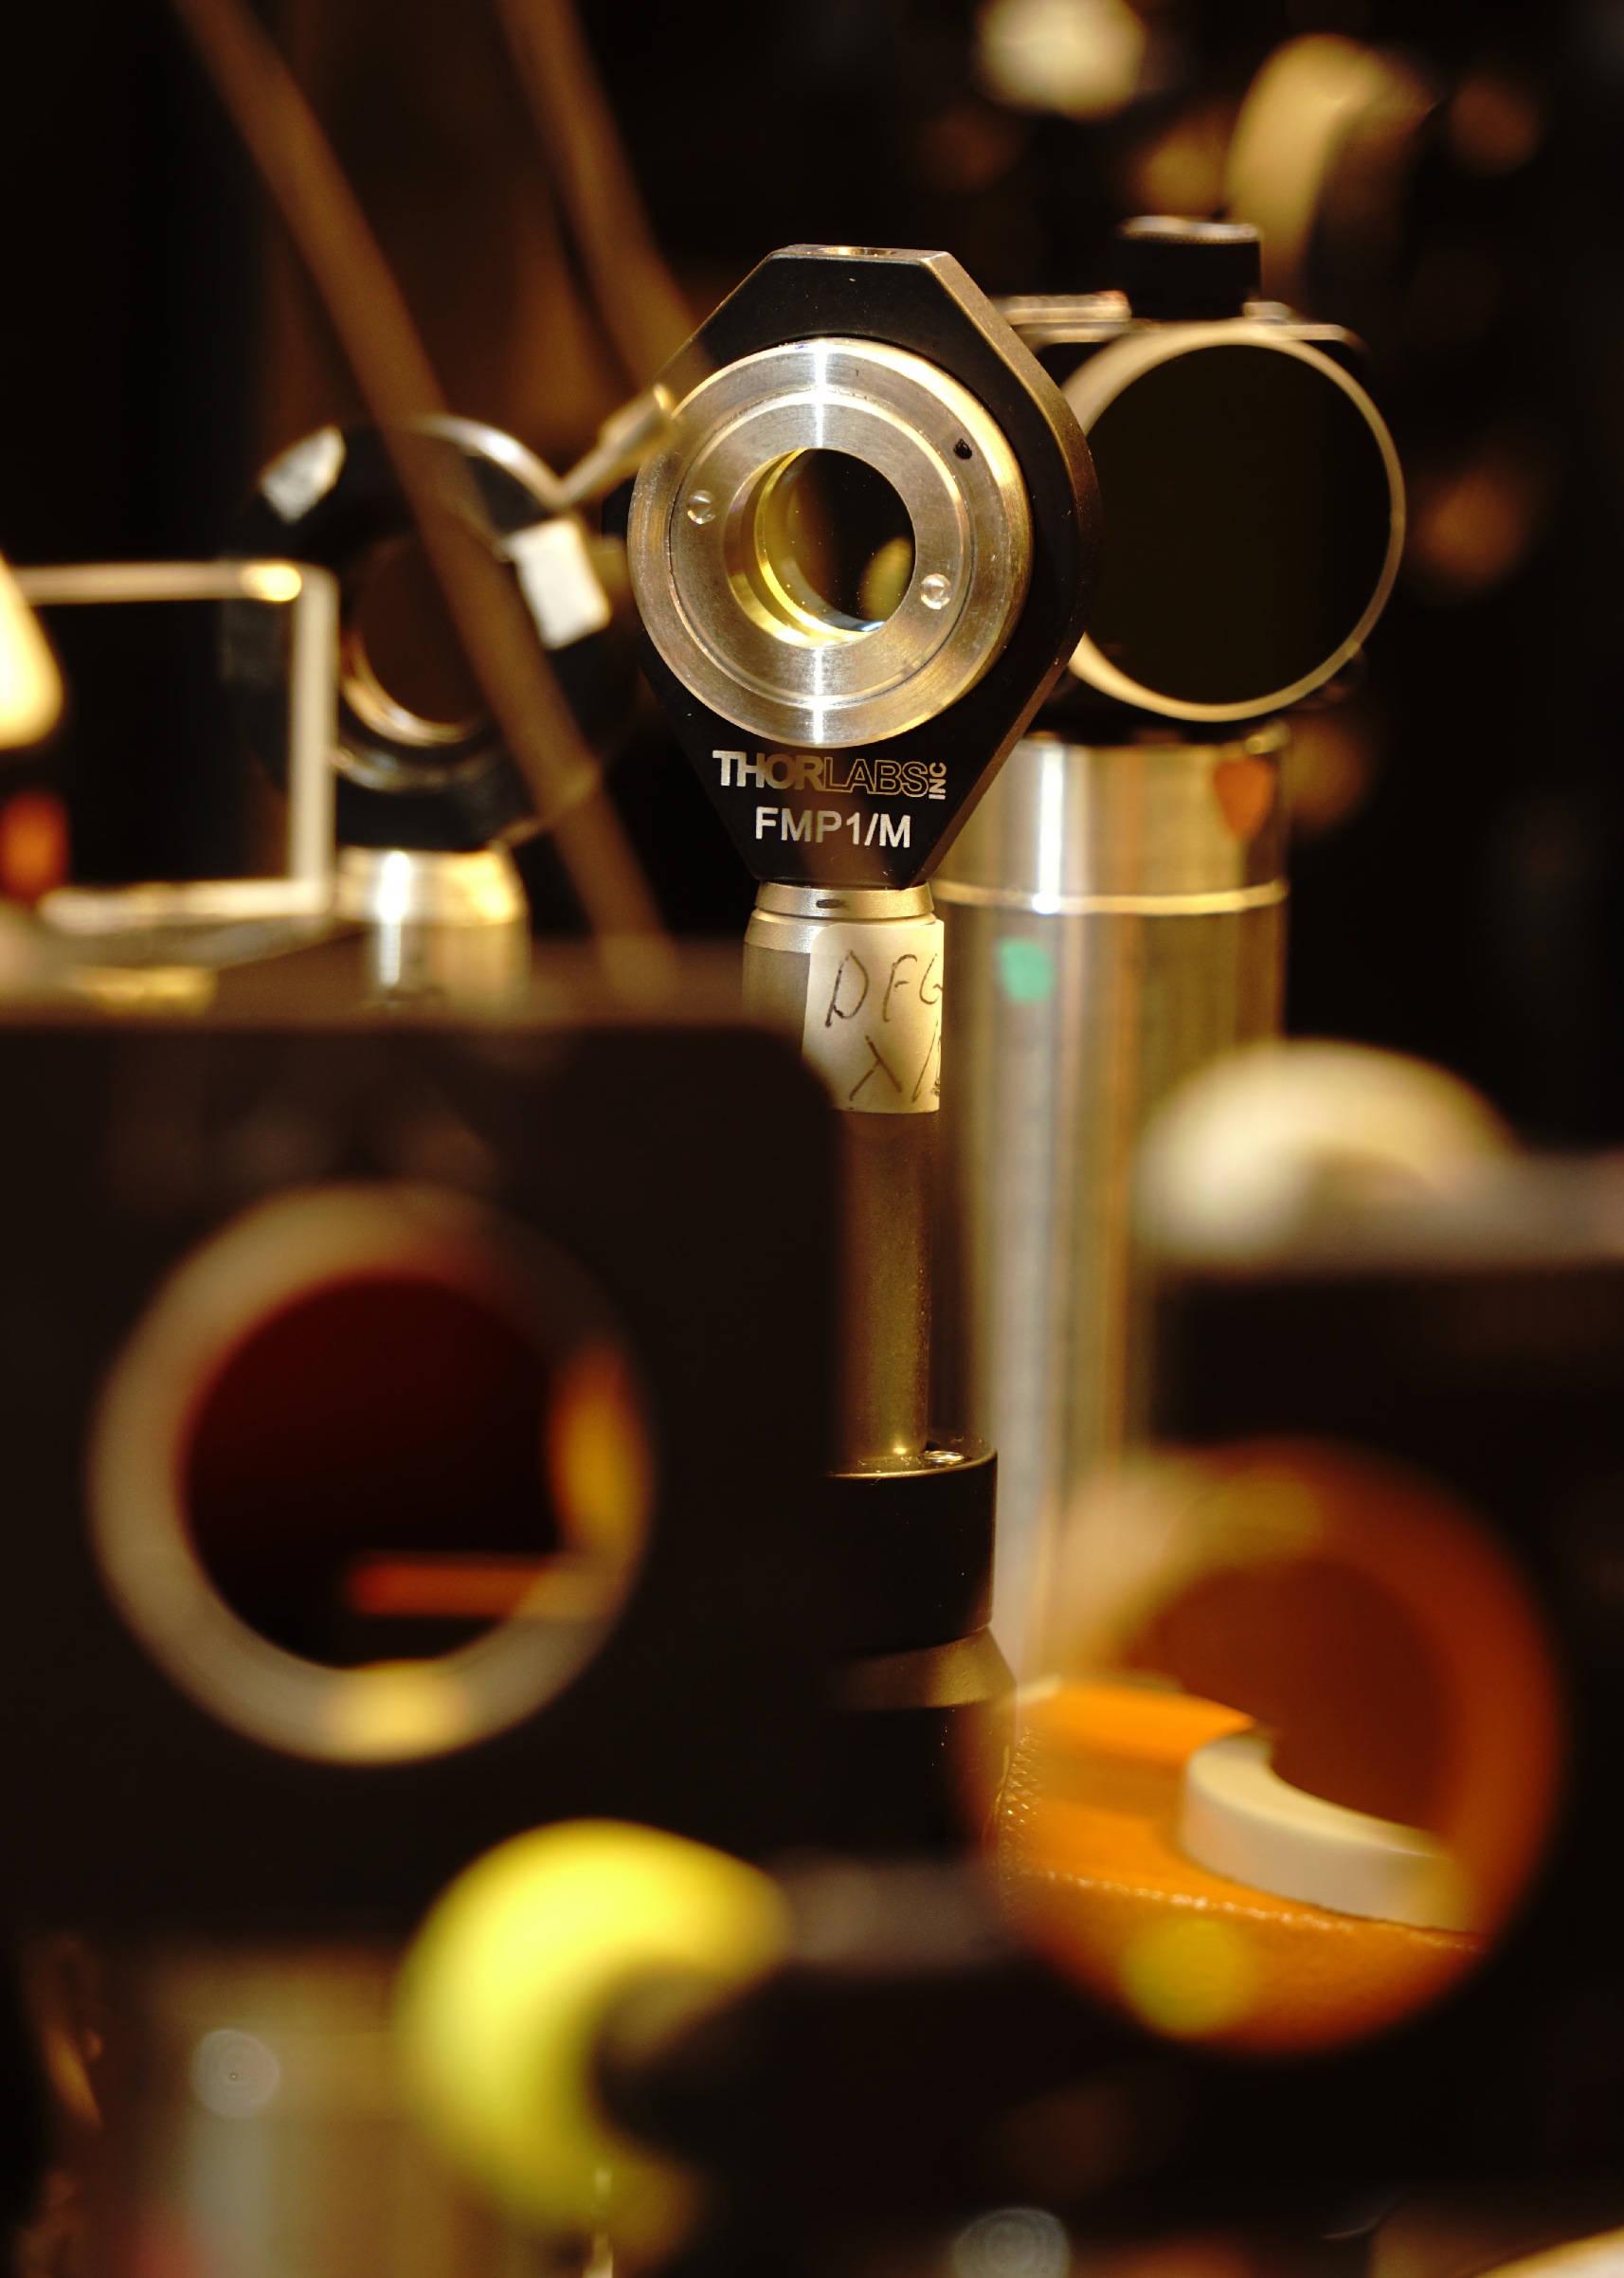
\includegraphics[width=\pdfpagewidth,height=\pdfpageheight]{fullpage_images/OpticsFig.pdf}};
%{\includegraphics[width=\pdfpagewidth,height=\pdfpageheight]{/Users/Cota/Documents/PhD/Thesis/ThesisRoberto/IMG/Chap3.pdf}};
\end{tikzpicture}

\clearpage



\begin{savequote}[75mm]
$\blacktriangleleft$ A \ce{ZnSe} window (the close field orange element in the bottom right) splits our laser pulses into a pump and a probe beam. A halfwave plate (at the focus of the image) enables us to change the polarization of our pump pulses. These two elements set the basis of polarization-resolved pump-probe spectroscopy, leading to a suitable method to observe molecular reorientation.
\end{savequote}




\chapter[Methods II: Vibrational spectroscopy]{Methods II\\Vibrational spectroscopy}
\label{chap:TRVS}
\label{ChapterTRVS}
\label{Chapter3}

\vspace{30pt}
	
	
In this chapter we discuss the theoretical background and experimental methodology used to study aqueous solutions by means of vibrational spectroscopy. In particular, we discuss the aspects that allow light to couple with molecular oscillators and to induce vibrational transitions. By targeting specific vibrational modes, we can then determine the connection between the observable macroscopic properties, such as absorption, and the underlying microscopic structure and dynamics.


\newpage	
	
\section{The classical harmonic oscillator}
	
%Rather than static structures, molecules are regarded as interconnected atoms that are constantly oscillating (small periodical displacements) around the positions that would minimize the internal energy. 
The simplest description of molecular vibrations starts from the classical approach of a diatomic molecule with masses $m$ and $M$ (with $M \gg m$). The two atoms are connected by a covalent chemical bond that acts as a spring, as shown in Figure~\ref{OscillatorsGen1}A. If $m$ experiences a small displacement with respect to its equilibrium position $x_0$ (i.e.\ the equilibrium bond length), the spring exerts a restoring force that follows Hooke's law with a spring constant $k$. Newton's second law states
\begin{eqnarray}
m \frac{d^2 x}{d t^2} + k x = 0,
\end{eqnarray}
with the solution 
\begin{eqnarray}
x (t) = x_0 \cos (\omega_0 t),
\end{eqnarray}
where $\omega_0 = \sqrt{k/m}$ is the frequency at which $m$ oscillates harmonically around its equilibrium position. The preceding equation describes the periodic displacement of $m$ bound to a much heavier atom.

Most molecules consist of more than two atoms. The intramolecular interactions are described as springs pairing all the atoms within the molecule (Fig.\ \ref{OscillatorsGen1}B). This means that the position of a given atom can be affected by multiple bonds, leading to more complex dynamics as compared to the previous example. For a molecule composed of $N$ atoms the equations of motion can be written as
\begin{eqnarray}
M \frac{d^2 X}{d t^2} +  K X = 0,
\label{GeneralizedVibration}
\end{eqnarray}
with $X$ a $3N$-element vector that describes the position of all masses in the three-dimensional space, and $M$ and $K$ matrices ($3N \times 3N$) that contain the corresponding masses $m_i$ and spring constants $k_{ji}$. 

Equation \ref{GeneralizedVibration} constitutes a set of coupled differential equations, which can be solved by a linear transformation to compute the eigenfrequencies of each oscillator in the molecule. We define a unitary matrix $U$ such that
\begin{eqnarray}
(M^{-1} K) U = U \Omega,
\label{EigenFunction1}
\end{eqnarray}
where $\Omega$ is a diagonal matrix that contains the eigenfrequencies $\omega_i$. The unitary matrix can also operate on $X$ to define a new vector as $Q = U^{-1} X$. Hence, Eq.\ \ref{GeneralizedVibration} can be diagonalized, and leads to the equation
\begin{eqnarray}
\frac{d^2 Q}{d t^2} +  \Omega Q = 0,
\label{Diagonalsolution}
\end{eqnarray}
that provides a set of $3N$ uncoupled differential equations. Hence, the oscillating dynamics of atoms within the molecule are described by superposition of independent harmonic oscillators $q_i$, conventionally called ``normal modes''.



\begin{figure}[t!]
	\centering
	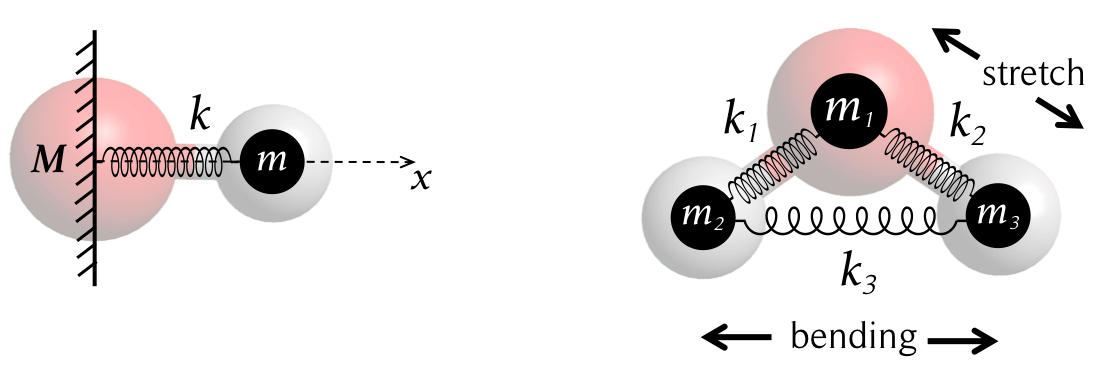
\includegraphics[width=0.85\figwidth]{chapters/Chapter3_Methods2/Graphs/Oscillators.png} %The local modes are calculated on the XXX level, and reproduced with permission from ref. XXX. 
	\caption{\textbf{Left:} Covalent chemical bonds can be modeled as harmonic oscillators. \textbf{Right:} Representation of a polyatomic molecule (water) with respect of its different degrees of vibrational freedom.}
	\label{OscillatorsGen1}
\end{figure}




Water molecules are formed by three atoms with two non-parallel covalent bonds, so water has three normal modes (see Fig.\ \ref{OscillatorsGen1}B): a bending mode, and two \ce{OH} stretches that combine to give the symmetric and antisymmetric stretch modes.\!\cite{Wang2004,Bakker2010,Perakis2016}



\section{Quantum description and vibrational transitions}


In the quantum mechanical description of molecular vibrations, we again describe chemical bonds as harmonic oscillators, leading to the following Hamiltonian:
\begin{eqnarray}
\hat{H}_0 = \frac{\hat{p}^2}{2m} + \frac{1}{2} k \hat{x}^2,
\label{SchodringerStatic}
\end{eqnarray} 
where $\hat{p}$ ($= -i \hslash \partial_x$) and $\hat{x}$ are the momentum and position operators. The first term represents the kinetic energy of the system, while the second corresponds to the potential energy of a particle in a Hooke's law-type potential. 

Solving the time-independent Schr\"odinger equation $\hat{H}_0 \ket{\Psi} = E \ket{\Psi}$ yields a family of solutions defined by the following orthogonal eigenstates 
\begin{eqnarray}
\ket{\psi_n (x)}=\frac{1}{\sqrt{2^{n} n !}} \cdot \left(\frac{m \omega_0}{\pi \hslash}\right)^{1 / 4} \cdot \exp \left(  {-\frac{ m \omega_0 x^{2}}{2 \hslash}}  \right) \cdot H_{n}\left(\sqrt{\frac{m \omega_0}{\hslash}} x \right),
\label{wavefunctions}
\end{eqnarray} 
with $\ket{\psi_{n}}$ the stationary wavefunctions that obey the relation $\braket{\psi_n}{\psi_m} = \delta_{nm}$, with $\delta_{nm}$ the Kronecker delta, and $H_n$ the Hermite polynomials. The corresponding eigenenergies are given by
\begin{eqnarray}
E_n = \hslash \omega_0 \left( n + \frac{1}{2}   \right), \qquad \text{with} \qquad n \in \mathbb{N}_0.
\label{eigenenergy}
\end{eqnarray}
\begin{figure}[t!]
	\centering
	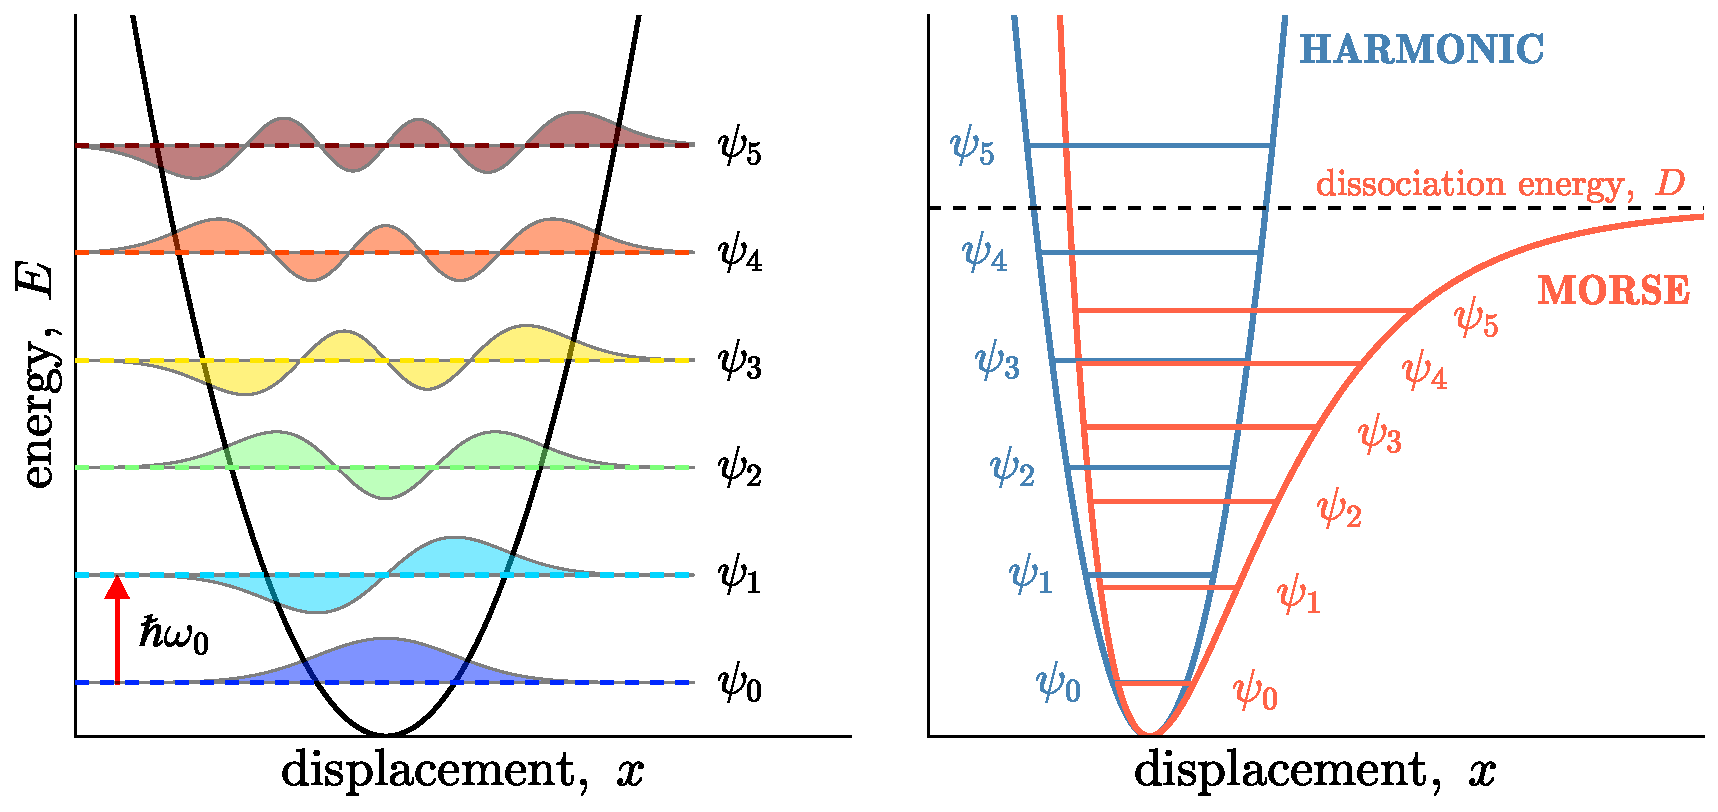
\includegraphics[width=1\figwidth]{chapters/Chapter3_Methods2/Graphs/PotentialHarmonicMorse.pdf} %The local modes are calculated on the XXX level, and reproduced with permission from ref. XXX. 
	\caption{\textbf{Left:} Wavefunctions described in a harmonic oscillator potential. Each wavefunction is drawn at its corresponding energy level. Consecutive level are equidistant by a quanta of energy $\hslash \omega_0$. \textbf{Right:} Comparison between the harmonic oscillator potential and anharmonic vibrations described by the Morse potential. Notice that the latter has a asymptotic behavior at large distances, which corresponds to the dissociation energy level. In the Morse potential, the space between consecutive energy levels decreases with increasing the quantum number $n$.}
	\label{PotentialsWaveFunctions}
\end{figure}

The value $n$ corresponds to the vibrational quantum number, and $\omega_0 = \sqrt{k/m}$. Eqs.\ \ref{wavefunctions} and \ref{eigenenergy} state that the energy is quantized and the system can only be in discrete states, referred to as zeroth, first, second and higher order vibrational states, shown in the left panel of Fig. \ref{PotentialsWaveFunctions}. From Eq.\ \ref{eigenenergy}, it is clear that the energy of the ground state ($n=0$) is not zero, but $E_0 = \hslash \omega_0 /2$ which is called the zero-point energy. Subsequent states are equidistantly separated by a quantum of energy $\hslash \omega_0$. 


%The discrete character of  contrast with the classical oscillator in which the ground state coincides with the static non-oscillating dynamics.





In the quantum description, transitions between levels can occur as the result of a time-dependent perturbation, such as light (electromagnetic waves). As shown in Eq.\ \ref{PotentialPolarization}, an electromagnetic wave interacts with the charges in the system, adding a new term to the Hamiltonian:
\begin{eqnarray}
\hat{H} = \hat{H}_0 + \hat{V}_\text{int}(t), \qquad \text{with} \qquad \hat{V}_\text{int}(t) = \hat{\vec{\mu}} \cdot \vec{E}(t),
\label{PerturbedHamiltonian}
\end{eqnarray} 
where $\vec{E}(t)$ refers to the electric field of the light and the dipole moment operator $\hat{\vec{\mu}}$ defines the distribution of charges $q$ in the system following $\hat{\vec{\mu}} = \sum_i q_i \hat{\vec{x}}_i$.


A transition from a vibrational level to another can be described using the time-dependent Schr\"odinger equation
\begin{eqnarray}
\hat{H} (t) \ket{\Psi} = i \hslash \frac{\partial}{\partial t} \ket{\Psi},
\label{TimeScrodinger}
\end{eqnarray} 
which can be solved by separation of variables. Using the expressions given by Eqs.\ \ref{wavefunctions} and \ref{eigenenergy}, the general solution to Eq.\ \ref{TimeScrodinger} is written as
\begin{eqnarray}
\ket{\Psi} = \sum_n c_n (t)  e^{  -i E_n t / \hslash  } \ket{\psi_n}
\label{GenSolTimeSchrodinger}
\end{eqnarray}
where $c_n (t)$ is the corresponding amplitude of each energy level at time $t$.


% and the probability of finding the system in any state $\ket{\psi_n}$ is found by evaluating
%the superposition of the different vibrational states given in Eq.\  and the different eigenenergies from Eq. , thus


Using Eqs.\ \ref{PerturbedHamiltonian}, \ref{TimeScrodinger} and \ref{GenSolTimeSchrodinger}, the time-dependent amplitude of a given $\ket{\psi_m}$ state can be computed as follows
\begin{eqnarray}
\frac{d }{d t} c_m (t) = \frac{1}{i \hslash} \sum_n c_n (t) \bra{\psi_m} \hat{V}_\text{int} \ket{\psi_n} e^{-i \omega_{nm} t},
\label{TransitionPsi}
\end{eqnarray}
where $\omega_{nm} = (E_n - E_m) / \hslash = - \omega_{mn}$ is the energy difference between the states $n$ and $m$. The preceding equation provides a full description of the population of the state $m$, although not practical because each unknown coefficient $c_m$ is determined by the whole set of $c_n$ coefficients. Assuming that the system is entirely in a single state $k$ at $t = 0$ and the initial state is negligibly perturbed over the time, meaning $c_k(0) = 1$ and $c_k(t) \simeq 1$, Eq.\ \ref{TransitionPsi} reduces to\!\cite{Sakurai1994}
\begin{eqnarray}
c_m (t) \simeq \frac{1}{i \hslash} \int_0^t \bra{\psi_m} \hat{V}_\text{int} (t') \ket{\psi_k} e^{-i \omega_{km} t'}.
\label{TransitionPsi2}
\end{eqnarray}

The simplest description of such perturbation is to assume a harmonically oscillating electric field (harmonic perturbation) as $\vec{E} = \vec{E}_0 [\exp(i \omega t) + \exp(-i \omega t)]$. In that case, the transition rate $\Gamma_{k \to m}$, that is defined as the time derivative of the square modulus of $c_m$, is given by 
\begin{eqnarray}
\Gamma_{k \to m} \simeq \frac{d}{d t} | c_m |^2 &=& \frac{2 \pi}{ \hslash^2} |   \bra{\psi_m} \hat{\vec{\mu}} \cdot \vec{E}_0 \ket{\psi_k}   |^2 \delta(  \omega \pm \omega_{km}), \nonumber \\
&=& \frac{2 \pi}{ \hslash^2} E_0^2 \cos^2 (\theta) |   \bra{\psi_m} \hat{\mu}  \ket{\psi_k}   |^2  \delta(\omega \pm \omega_{km} ),
\label{TransRate}
\end{eqnarray}
which is the so-called Fermi's golden rule, where $\theta$ defines the angle between the dipole moment and the polarization of the perturbing electric field. The expression $ \mu_{mk} = \bra{\psi_m} \hat{\mu}  \ket{\psi_k}$ is generally called transition dipole moment. In the last expression, the dipole operator $\hat{\mu}$ refers to the entire distribution of charges, which encompasses transition dipoles of any kind. In the case of vibrational transitions, the transition dipole operator can be written in terms of the oscillation coordinate $x$ and the equilibrium position $x_0$ by the following expansion
\begin{eqnarray}
\hat{\mu} = {\mu}_0 + \frac{d {\mu}}{ d x} (\hat{x} - {x}_0) + \cdots
\end{eqnarray}
which leads to 
\begin{eqnarray}
\Gamma_{k \to m} = \frac{2 \pi}{ \hslash^2} E_0^2 \cos^2 (\theta) \left( \frac{d \mu}{d x}   \right)^2 |   \bra{\psi_m} \hat{x}  \ket{\psi_k}   |^2  \delta(\omega \pm \omega_{km} ).
\label{TransRateFinal}
\end{eqnarray}

This equation has the following physical interpretation: 

\begin{itemize}
	\item {The $\delta(\omega \pm \omega_{km})$ term represents the conservation of energy in the transition $\ket{\psi_k} \to \ket{\psi_m}$. We see that such condition can only be satisfied either by energy taken away from the external electric field (absorption if $E_m \simeq E_k + \hslash \omega$) or by energy given out to the external electric field (stimulated emission if $E_m \simeq E_k - \hslash \omega$). In both cases, such transition takes place when $\omega$ matches the energy difference between the states $m$ and $k$ (see Fig.\ \ref{dia2})}.
	\item {The $\bra{\psi_m} \hat{x}  \ket{\psi_k} $ term establishes the transition selection rule since it is zero unless $m = k \pm 1$, meaning that transitions only occur between consecutive states.\!\cite{Sakurai1994}}
\end{itemize}
	\begin{figure}[t!]%* is used because without it the figure does not appear
		\centering	
		\begin{tikzpicture}[>=stealth,thick,photon/.style={decorate,decoration={snake,post length=1.3mm}}]	
		
	
		\draw[->, line width=0.6mm, ForestGreens] (4.4-4,2.4) -- (4.4-4,4.0);		
		
		\draw[black,line width=0.7mm](3.8-4,4.0) -- (5-4,4.0) node[right] {$\ket{\psi_{n+1}}$};
		\draw[black,line width=0.7mm](3.8-4,2.4) -- (5-4,2.4) node[right] {$\ket{\psi_{n}}$};
				
		\draw[->,photon, line width=0.4mm, red] (2.9-4,3.2) -- (4.3-4,3.2) node[pos=0.2, above] {$\hslash \omega_0$};

		
		
		
		
		\draw[->, line width=0.6mm, blue] (4.4,4.0) -- (4.4,2.4);		
		
		\draw[black,line width=0.7mm](3.8,4.0) -- (5,4.0) node[right] {$\ket{\psi_{n+1}}$};
		\draw[black,line width=0.7mm](3.8,2.4) -- (5,2.4) node[right] {$\ket{\psi_{n}}$};
		
		\draw[->,photon, line width=0.4mm, red] (2.9,3.2) -- (4.3,3.2) node[pos=0.2, above] {$\hslash \omega_0$};
		
		\draw[->,photon, line width=0.4mm, red] (4.6,3.4) -- (6.0,3.4) node[pos=0.2, above] {$\hslash \omega_0$};	
		
		\draw[->,photon, line width=0.4mm, red] (4.6,3.0) -- (6.0,3.0) node[pos=0.2, below] {$\hslash \omega_0$};
		
			
			
			
		\draw[->, photon, line width=0.5mm, MyYellow] (4.4+4,4.0) -- (4.4+4,2.4);			
			
		\draw[black,line width=0.7mm](3.8+4,4.0) -- (5+4,4.0) node[right] {$\ket{\psi_{n+1}}$};
		\draw[black,line width=0.7mm](3.8+4,2.4) -- (5+4,2.4) node[right] {$\ket{\psi_{n}}$};
		
		%\draw[->,photon, line width=0.4mm, red] (4.6+4,3.2) -- (6.0+4,3.2) node[pos=0.2, above] {$\hslash \omega_0$};	
		
%		\draw[black,line width=1.2mm](3.5,1.0) -- (5.0,1.0) node[pos=0.5,below] {hot ground state};
		
%		\draw[black,line width=1.2mm] (1,0.2) -- (7,0.2) node[pos=0.15,above] {ground state};
		
		
		\node[right,fill=white,opacity=.2,text opacity=1,align=left] at (3.5-4,1.625) {$\text{absorption}$};
		
		\node[right,fill=white,opacity=.2,text opacity=1,align=left] at (3.5,1.8) {$\text{stimulated}$};
		\node[right,fill=white,opacity=.2,text opacity=1,align=left] at (3.65,1.45) {$\text{emission}$};
		
		\node[right,fill=white,opacity=.2,text opacity=1,align=left] at (3.4+4,1.8) {$\text{spontaneous}$};
		\node[right,fill=white,opacity=.2,text opacity=1,align=left] at (3.8+4,1.45) {$\text{decay}$};

		
%		\draw[white,line width=0.05mm](1,-0.1) -- (7,-0.1);
		
		
		\end{tikzpicture}		
		\caption{Illustration for three different transition processes: absorption, stimulated emission and spontaneous decay. The illustration pictures the ideal case in which the energy of the photon matches the energy difference between two consecutive states.}
		\label{dia2}			
	\end{figure}
\begin{itemize}
	\item {The $d \mu / d x$ term implies that the external electric field only couples to those vibrations that induce changes in the dipole moment.}
	\item {From the term $\cos^2 (\theta)$, we observe that the probability of a $\ket{\psi_k} \to \ket{\psi_m}$ transition to occur depends on the angle between the transition dipole moment and the polarization of the external electric field. This probability is maximal at $\theta = 0$, which means $ \vec{\mu} \parallel \vec{E}_0$. This is the basis of polarization-resolved spectroscopy which we will discuss later.}
\end{itemize}


In real molecules, the potential cannot be quadratic due to molecular dissociation at large interatomic distances.\!\cite{Maksyutenko2012} A more adequate potential to include the effect of molecular dissociation is given by
\begin{eqnarray}
V_\text{M} (x) = D \left( 1 - e^{-a x}   \right)^2,
\label{MorsePotential}
\end{eqnarray}
the so-called Morse potential,\!\cite{Morse1929} shown in the right panel of Figure~\ref{PotentialsWaveFunctions}. The energy at which the bond dissociates is represented by $D$, and $a = \sqrt{k/2D}$ the width of the potential. By introducing Eq.\ \ref{MorsePotential} in Eq.\ \ref{SchodringerStatic} instead of the harmonic oscillator potential, the corresponding eigenenergies related to the Morse potential are expressed as follows
\begin{eqnarray}
E_n = \hslash \omega_0 \left( n + \frac{1}{2}   \right) - \frac{\hslash^2 \omega_0^2}{4 D} \left( n + \frac{1}{2}   \right)^2,
\label{MorseEnergies}
\end{eqnarray}
where $n$ again is the vibrational quantum number and the angular frequency $\omega_0$ ($= \sqrt{k/m}$) satisfies also the relation $ \omega_0 = a \sqrt{2 D/ m}$. In contrast to the description of an harmonic oscillator, the energy separation between consecutive states becomes smaller with increasing the quantum number $n$. At low $n$, Eq.\ \ref{MorseEnergies} can be well represented by Eq.\ \ref{eigenenergy}. Further potentials have been explored to overcome some limitations of the Morse potential, such as the long-range Morse potential that captures the attractive long-range behavior in real systems.\!\cite{LeRoy2009}





\section{Linear absorption spectroscopy}


The way in which light interacts with an absorbing medium can give information at the molecular level. As in the previous chapter, to describe the vibrational experiments we need to construct models based on the changes that an incident field (light) experiences as it propagates through a medium. 

Assume a system of molecular oscillators of the same species in thermal equilibrium, meaning that the system is isotropic and in the ground state $\ket{0}$, so absorption is the most likely process to occur in the presence of light. This process will lead to attenuation of the incident field and non-zero, but relatively small, population of the first excited state $\ket{1}$.

For monochromatic light with intensity of $I_0 = c \epsilon_0 |E_0|^2 /2$ and frequency $\omega$, the absorbed power associated with the $\ket{0} \to \ket{1}$ transition is written as $P_\text{01} = \hslash \omega \Gamma_{0 \to 1}$. The absorption cross section $\sigma_\text{10}$ is defined as the ratio between the latter expressions, and using Eq.\ \ref{TransRateFinal}, is given by
\begin{eqnarray}
\sigma_\text{10} (\omega) = \frac{P_\text{10} (\omega) }{I_0} =  \frac{\pi \omega }{3 c \epsilon_0 \hslash } \mu_{10} \delta(\omega \pm \omega_{10})
\label{crosssection}
\end{eqnarray}
in which $\langle cos^2 \theta \rangle = 1/3 $ since the material is assumed isotropic. The cross section can be understood as an effective transverse area (not necessarily linked to the dimensions of the molecule) that the incident field must hit in order for the given transition to occur.

Assume now that a field propagates in the $z$ direction through a material with thickness $L$ and density of oscillators in the ground state $\rho$ (Fig.\ \ref{AbsorptionLambertBeer}), the Lambert-Beer law
\begin{eqnarray}
d I = - \sigma_\text{10} (\omega) \rho I {d z}
\label{lambertbeerlaw}
\end{eqnarray}
states that the variation of intensity $d I$ through propagation in a segment $dz$ is equal to the product between the intensity and the cross section of the material. Integrating this expression gives
\begin{eqnarray}
I = I_0 \exp [- \beta (\omega) L ],
\label{lambertbeerlaw2}
\end{eqnarray}
\begin{figure}[t!]
	\centering
	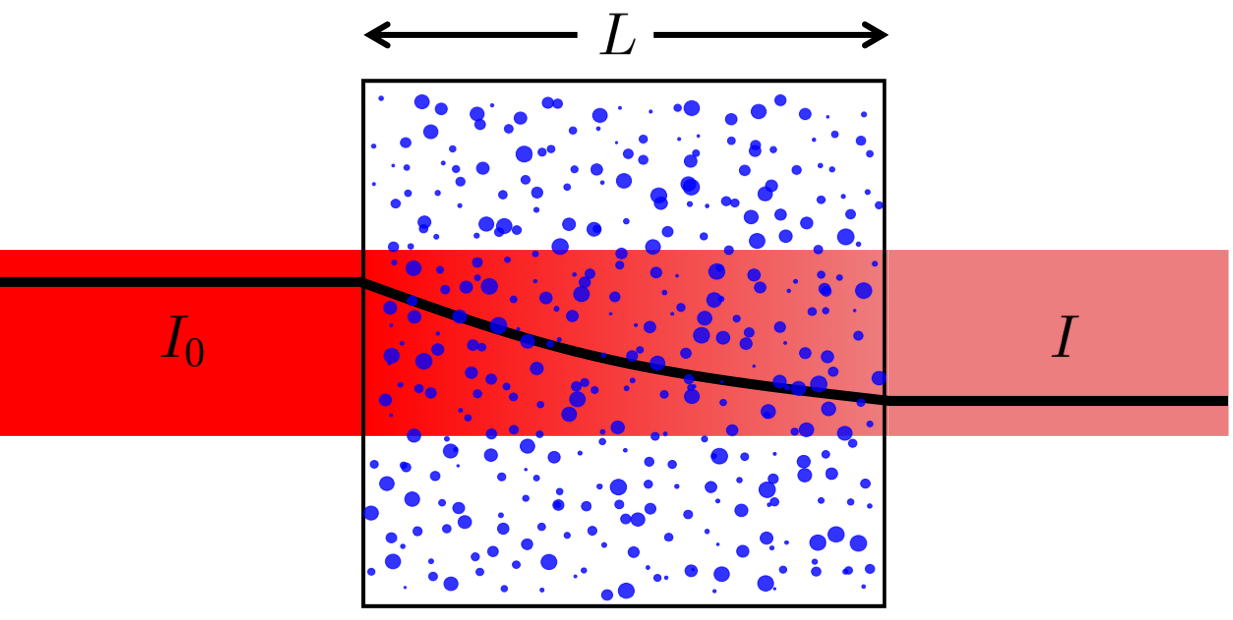
\includegraphics[width=0.6\figwidth]{chapters/Chapter3_Methods2/Graphs/LambertBeerAbs.png} %The local modes are calculated on the XXX level, and reproduced with permission from ref. XXX. 
	\caption{In linear absorption spectroscopy, one studies the decrement on the intensity of light as it propagates through a material. The initial and the final intensities are linked by the spectroscopic properties of the sample as described by Eqs.\ \ref{crosssection} and \ref{lambertbeerlaw2}.}
	\label{AbsorptionLambertBeer}
\end{figure}
\noindent with $\beta (\omega) = \rho \sigma_\text{10} (\omega)$ the attenuation coefficient. This equation provides a link between the macroscopic transmission of the material, $T = I/I_o$, with the microscopic molecular property $\sigma_{10}$. The absorbance, which provides a more convenient and linear relation between the relevant parameters, is given by
\begin{eqnarray}
\alpha (\omega) = - \ln \frac{I}{I_0} = \sigma_{10} (\omega) \rho L.
\label{absorbance}
\end{eqnarray}




As can be observed from Eq.\ \ref{crosssection}, a vibrational transition will only occur when the frequency of the electric field matches the energy difference between the excited and ground states. 


In condensed-phase systems, the absorption spectrum $\alpha(\omega)$ is not a delta function as it would result from Eqs.\ \ref{crosssection} and \ref{absorbance}, but has a finite width. This is due to two effects. First, the finite excited-state lifetime and fast fluctuations in the resonance frequency (due to interaction of the oscillator with its surroundings) give rise to so-called homogeneous broadening. This broadening occurs for each individual oscillator, and if all oscillators have the same resonance frequency $\omega_{10}$, it typically gives rise to a Lorentzian line shape:
\begin{eqnarray}
I (\omega ) \propto \frac{1}{\pi} \frac{\gamma/2}{ (\omega - \omega_{10})^2 + (\gamma/2)^2},
\label{Lorentzian}
\end{eqnarray}
where $\gamma$ is the homogeneous line width (see Fig.\ \ref{BroadeningFigure1}-left). In addition, there may exist a distribution of resonance frequencies $\omega_{10}$ in the sample, so that the absorption spectrum becomes the convolution of Eq.\ \ref{Lorentzian} with this distribution of resonance frequencies (see Fig.\ \ref{BroadeningFigure1}-right). This so-called inhomogeneous broadening occurs very often in hydrogen-bonded systems, where local differences in hydrogen-bond strength give rise to a broad distribution of \ce{OH}- or \ce{OD}-stretch frequencies (see Chapters \ref{ChapterHydroxide}, \ref{ChapterForster} and \ref{ChapterPhenolate}).



\begin{figure}[t!]
	\centering
	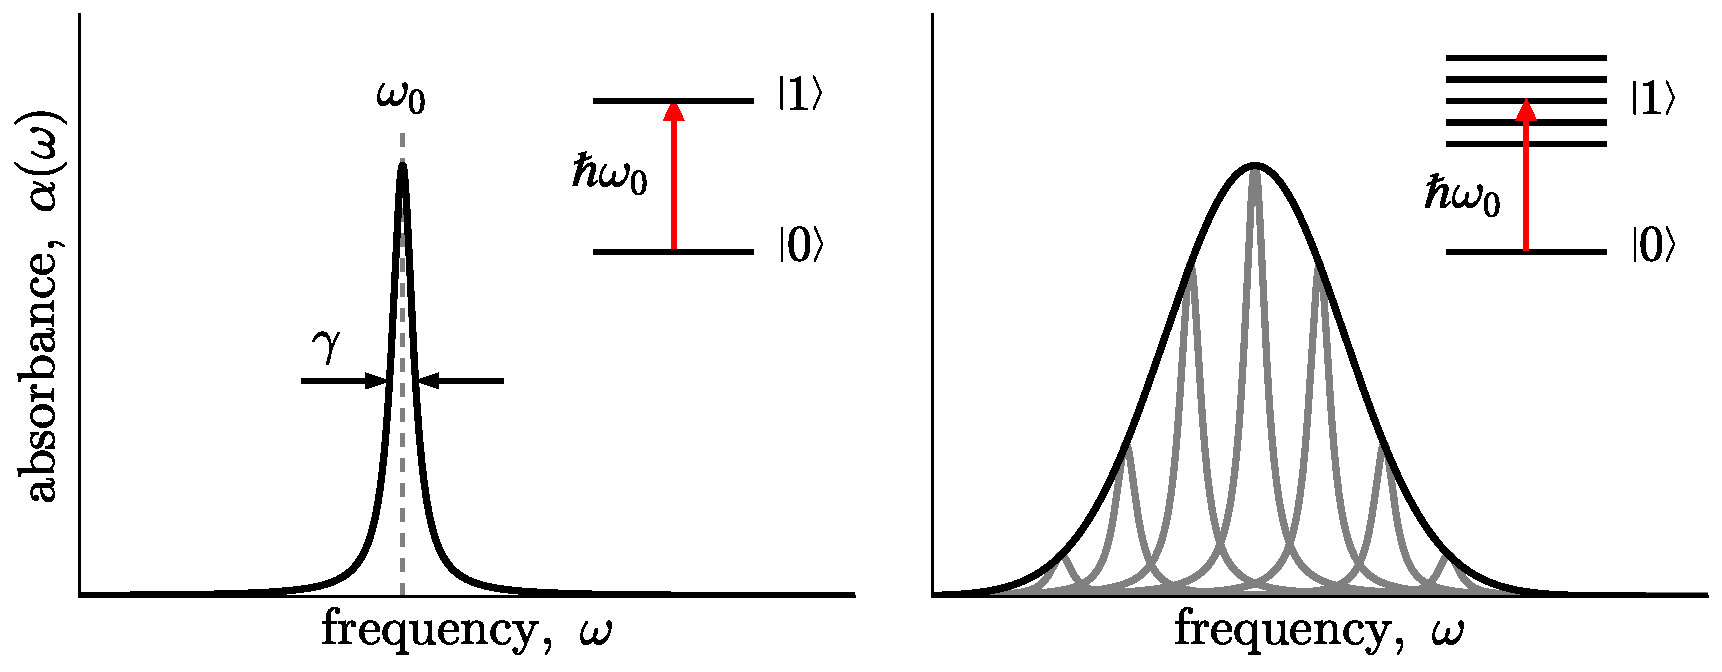
\includegraphics[width=0.95\figwidth]{chapters/Chapter3_Methods2/Graphs/LineShape.pdf} %The local modes are calculated on the XXX level, and reproduced with permission from ref. XXX. 
	\caption{\textbf{Left:} homogeneous broadening due to the finite lifetime of the excited state and fast fluctuations of the resonance frequency. This effect follows a Lorentzian functional form.  \textbf{Right:} the absorption lineshape is further broadened due to intermolecular interactions such as hydrogen bonding, leading to a statistical distribution of the resonance frequency.}
	\label{BroadeningFigure1}
\end{figure}





\section{Time-resolved vibrational spectroscopy}\label{TRVSExp}

Pump-probe spectroscopy is a useful tool to study dynamical aspects of molecular systems. This technique is based on an intense pulse that excites a significant fraction of the oscillators contained in a sample to the excited state (pump), while a second time-delayed weak pulse monitors the equilibration mechanism of the excited oscillators (probe). The pump and probe processes are shown in Figure~\ref{excitationscheme}.


\begin{figure}[t!]%* is used because without it the figure does not appear
	\centering	
	\begin{tikzpicture}[>=stealth,thick,photon/.style={decorate,decoration={snake,post length=1.3mm}}]	
	
	
	\draw[black,line width=0.6mm](3-6,5.0) -- (4.9-6,5.0) node[right] {$\ket{2}$};
	\draw[black,line width=0.6mm](3-6,4.0) -- (4.9-6,4.0) node[right] {$\ket{1}$};
	\draw[black,line width=0.6mm](3-6,2.7) -- (4.9-6,2.7) node[right] {$\ket{0}$};
	
	
	\draw[->, line width=0.6mm, ForestGreens] (3.7-6,2.7) -- (3.7-6,4.0);
	\draw[->, line width=0.6mm, ForestGreens] (4.2-6,2.7) -- (4.2-6,4.0);
	\draw[->, line width=0.6mm, ForestGreens] (4.45-6,2.7) -- (4.45-6,4.0);	
	
	
	\filldraw[gray] (3.2-6,2.7) circle (3pt);
	\filldraw[gray] (3.45-6,2.7) circle (3pt);	
	\filldraw[gray] (3.7-6,2.7) circle (3pt);	
	\filldraw[gray] (3.95-6,2.7) circle (3pt);	
	\filldraw[gray] (4.2-6,2.7) circle (3pt);	
	\filldraw[gray] (4.45-6,2.7) circle (3pt);	
	\filldraw[gray] (4.7-6,2.7) circle (3pt);	
	
	
	\draw[->,photon, line width=0.4mm, red] (1.2-6,4.7) -- (2.6-6,4.2);
	
	\draw[->,photon, line width=0.4mm, red] (1.2-6,4.4) -- (2.6-6,3.9);	
	
	\draw[->,photon, line width=0.4mm, red] (1.2-6,4.1) -- (2.6-6,3.6);
	
	\node[right,fill=white,opacity=.2,text opacity=1,align=left] at (1.3-6,3.3) {$\text{pump}$};
	
	
	
	
	
	\draw[black,line width=0.6mm](3,5.0) -- (4.9,5.0) node[right] {$\ket{2}$};
	\draw[black,line width=0.6mm](3,4.0) -- (4.9,4.0) node[right] {$\ket{1}$};
	\draw[black,line width=0.6mm](3,2.7) -- (4.9,2.7) node[right] {$\ket{0}$};
	
	\draw[->, line width=0.6mm, ForestGreens] (3.45,2.7) -- (3.45,4.0);
	\draw[->, line width=0.6mm, ForestGreens] (3.7,4.0) -- (3.7,5.0);
	\draw[->, line width=0.6mm, blue] (4.2,4.0) -- (4.2,2.71);	
	
	
	\filldraw[gray] (3.2,2.7) circle (3pt);
	\filldraw[gray] (3.45,2.7) circle (3pt);	
	\filldraw[gray] (3.7,4.0) circle (3pt);	
	\filldraw[gray] (3.95,2.7) circle (3pt);	
	\filldraw[gray] (4.2,4.0) circle (3pt);	
	\filldraw[gray] (4.45,4.0) circle (3pt);	
	\filldraw[gray] (4.7,2.7) circle (3pt);	
	
	%	\draw[->,photon, line width=0.4mm, red] (1.2,4.7) -- (2.6,4.2);
	
	\draw[->,photon, line width=0.4mm, red] (1.2,4.4) -- (2.6,3.9);	
	
	%	\draw[->,photon, line width=0.4mm, red] (1.2,4.1) -- (2.6,3.6);
	
	\node[right,fill=white,opacity=.2,text opacity=1,align=left] at (1.3,3.6) {$\text{probe}$};
	
	\end{tikzpicture}		
	\caption{Illustration of pump-probe spectroscopy in which the first three vibrational states are considered. The gray circles represent population. \textbf{Left:} at $t = 0$, an intense pump beam promotes vibrations to the first excited state (green arrows), which are after monitored by a second beam called probe. \textbf{Right:} the probe induces three different effects: excitation from ground to the first excited state, excitation from the first to the second excited state, and stimulated emission from the first to the ground state.}
	\label{excitationscheme}			
\end{figure}


Here, we aim to provide a phenomenological understanding behind pump-probe spectroscopy. To this purpose, we start with the notion of transient absorption which arises from the difference between the absorption of the perturbed sample and of the unperturbed sample. The system is perturbed out of its equilibrium due to te intense pump pulse. The transient absorption is defined as
\begin{eqnarray}
\Delta \alpha (\omega,t) = \alpha_\text{p} (\omega,t) - \alpha_\text{u}(\omega),
\label{transientspectra1}
\end{eqnarray} 
where the subindices $p$ and $u$ refer to the pumped and the unpumped sample. As shown in Eq.\ \ref{absorbance}, the absorbance of the unpumped sample is given by
\begin{eqnarray}
\alpha_\text{u} (\omega) = \sigma_{01} (\omega) N_0
\end{eqnarray}
with $N_0 = \rho L$ the number of vibrational absorbers per area unit in the ground state. After excitation by the pump pulse, the prope pulse will experience a change in the absorption as the result of three different processes. First, the density of absorbers in the ground state is reduced, such that the $\ket{0} \to \ket{1}$ absorption is reduced by a factor of $(N_0-N_1(t))/N_0$, with $N_1(t)$ the density of molecules in the excited state at any time. A second effect is stimulated emission that also manifests itself as an increase in the transmission of the sample, in other words, a reduced absorbance according to Eq.\ \ref{absorbance}. Third, the probe pulse can promote molecules from the first to the second excited state which induces an absorption matching the $\ket{1} \to \ket{2}$ transition. These effects can be represented as follows
\begin{eqnarray}
\alpha_\text{p} (\omega,t) = \underbrace{\sigma_{10} (\omega) [N_0 - N_1(t)]}_{\text{ground state} \atop \text{depletion}}  - \underbrace{\sigma_{01} (\omega) N_1(t)}_{\text{stimulated} \atop \text{emission}} + \underbrace{\sigma_{21} (\omega) N_1 (t)}_{\text{induced} \atop \text{absorption}}.
\end{eqnarray}
Since $\sigma_{10} = \sigma_{01}$, the transient absorption change defined in Eq.\ \ref{transientspectra1} reduces to
\begin{eqnarray}
\Delta \alpha (\omega,t) = - \underbrace{ 2 \sigma_{10} (\omega) N_1(t)}_{\text{bleaching} \atop \text{band}} + \underbrace{\sigma_{21} (\omega) N_1 (t)}_{\text{induced} \atop \text{absorption}}, 
\label{transientabs2}
\end{eqnarray}
with features that are represented in the left side of Figure~\ref{TRVSAspects1} (for short time delays).


\begin{figure}[t!]
	\centering
	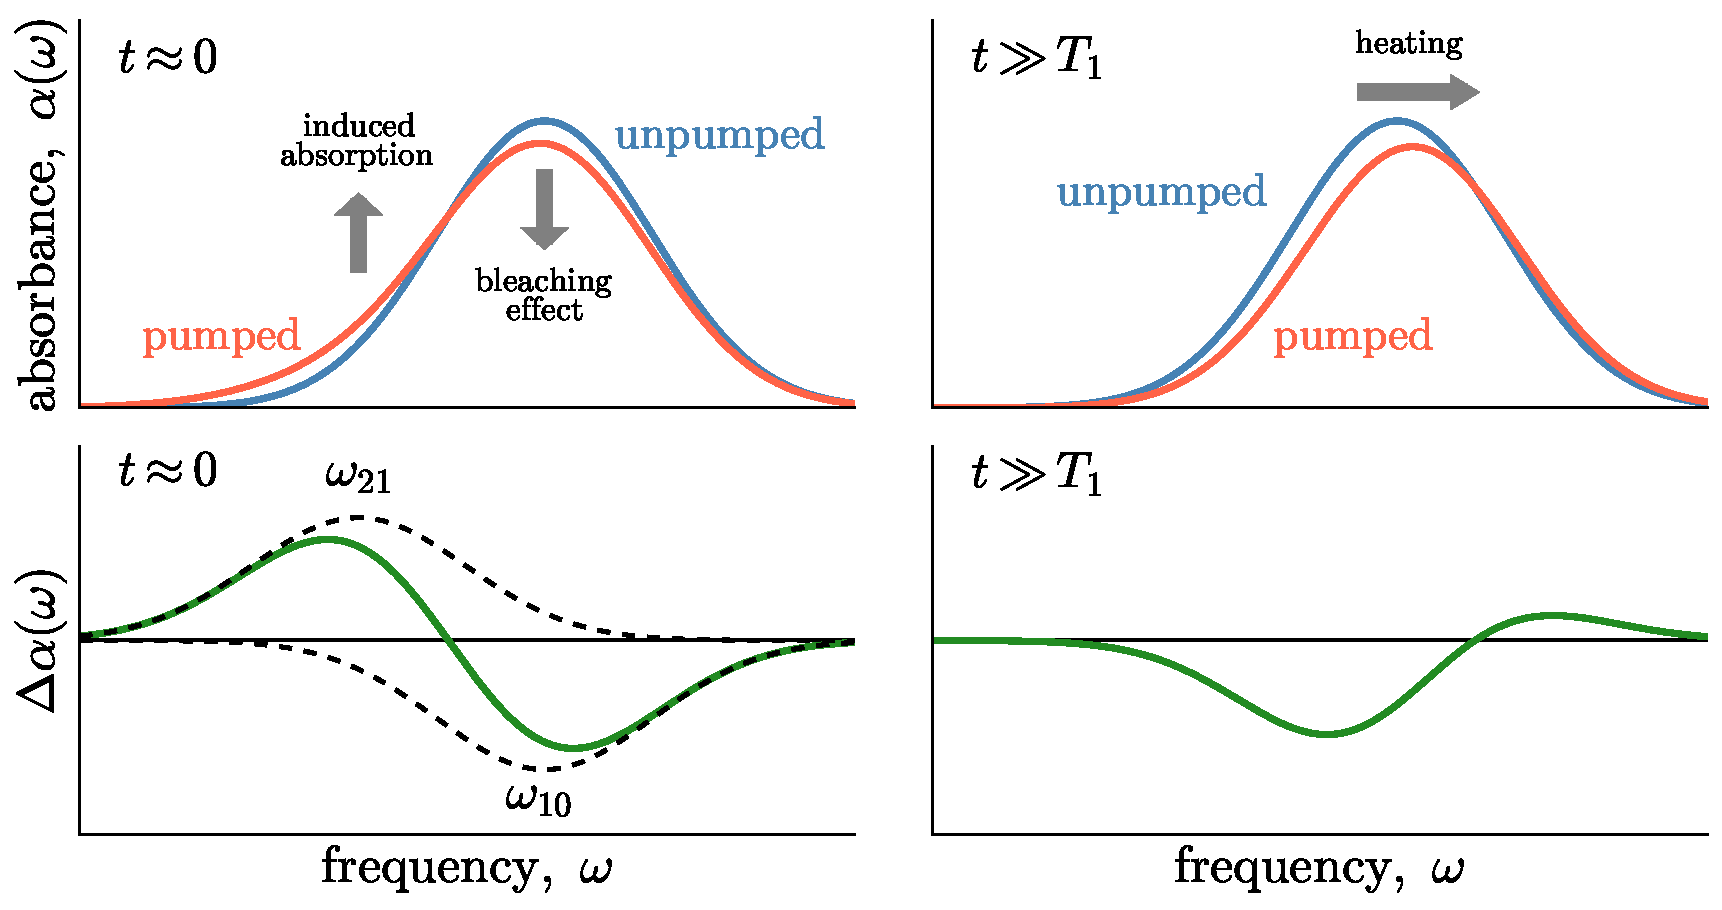
\includegraphics[width=0.95\figwidth]{chapters/Chapter3_Methods2/Graphs/TRVSAspects.pdf} %The local modes are calculated on the XXX level, and reproduced with permission from ref. XXX. 
	\caption{Illustration of pump-probe spectra that resemble the response of the \ce{OD} stretch vibration of \ce{HDO} molecules isotopically diluted in \ce{H2O}. \textbf{Left:} at short time delays the absorption is reduced around $\omega_{10}$ (bleaching), while absorption around $\omega_{21}$ is accessible. \textbf{Right:} at long time delays the absorption spectrum shifts to the blue and reduces in amplitude due to temperature increase upon vibrational relaxation.}
	\label{TRVSAspects1}
\end{figure}



In the simplest scenario, the excited molecules decay directly to the ground state, so that the bleaching and induced absorption vanish exponentially in the same fashion, such that
\begin{eqnarray}
\Delta \alpha (\omega,t) = [ -  2 \sigma_{10} (\omega) + \sigma_{21}(\omega)] N_1 (0) e^{-t/T_1},
\label{transientabs3}
\end{eqnarray}
with $T_1$ the lifetime of the vibrationally excited state. In general, the lifetime represents the equilibration rate of the excited vibration with respect to its surroundings. 









In Chapter \ref{ChapterHydroxide}, we show that \ce{OD} stretches hydrating hydroxide ions relax much faster ($\sim$0.3 ps) than those in neat water with vibrational lifetime of 1.7 ps. The accelerated equilibration rate is associated to the strong hydrogen bonds in the immediate ionic vicinity. This type of dynamical variations, along with spectral differences, allow us to disentangle different spectral contributions in a way that is not possible with linear absorption spectroscopy. This separation has been widely used to interrogate the behavior of molecules in different environments, as shown in Chapters \ref{ChapterHydroxide}, \ref{ChapterForster} and \ref{ChapterPhenolate}.

In aqueous solutions, vibrational energy relaxation may follow more complicated relaxation pathways that involve intermediate states, and in the presence of solutes, different modes that overlap spectrally may be excited simultaneously, as we will see in Chapters \ref{ChapterHydroxide} and \ref{ChapterForster}.


  

\section{Polarization-resolved pump-probe spectroscopy}\label{Eqs_PR-TRVS}


The assumption of having an isotropic system in thermal equilibrium holds valid, until the pumped pulse, which in our case is linearly polarized, interacts with the system. As has been discussed before, Eq.\ \ref{TransRateFinal} shows that light couples primarily with transition dipole moments aligned parallel to the polarization of the electric field. In fact, this polarization-dependent absorption will induce an anisotropy in the distribution of excited oscillators that can be used to explore molecular reorientation, which is intimately linked to structural properties. 


Once again, let us assume a system of molecules that show an isotropic distribution. Immediately after excitation, the normalized distribution of excited vibrations is given by
\begin{eqnarray}
p(\theta,\phi,t=0) = \frac{3}{4 \pi} \cos^2 (\theta)
\label{distributionexcitestate}
\end{eqnarray}
with $\theta$ the polar and $\phi$ the azimuthal angles with respect of the pump polarization. Hence, probing the sample in polarization parallel or perpendicular to that of the pump will delivers a polarization-dependent transient absorption. 


If we define our coordinate system with the pump light propagating along the $x$ axis with its polarization along the $z$ axis, it follows to the parallel (z-polarization) and perpendicular (y-polarization) transient signals described by
\begin{eqnarray}
\Delta \alpha_\parallel (\omega, t) &=& 3 \Delta\sigma (\omega) N_1 (t) \int_S p(\theta,\phi,t) \cos^2 (\theta) dS \\
\Delta \alpha_\perp (\omega, t) &=& 3 \Delta\sigma (\omega) N_1(t) \int_S p(\theta,\phi,t) \sin^2 (\theta) \sin^2 (\phi) dS
\end{eqnarray}
where the integral runs over the surface of the unit sphere. The term $\Delta\sigma (\omega) = -2 \sigma_{10}(\omega) + \sigma_{21}(\omega) $ is the (theoretical) isotropic cross section which encompasses the bleaching band and induced absorption, see Eq.\ \ref{transientabs2}. By explicitly solving the integrals using Eq.\ \ref{distributionexcitestate}, we find the initial parallel and perpendicular signals in terms of the isotropic response as
\begin{eqnarray}
\Delta \alpha_\parallel (\omega, 0) = \frac{9}{5} \Delta\sigma (\omega) N_1 (0) \qquad \text{and} \qquad \Delta \alpha_\perp (\omega, 0) = \frac{3}{5} \Delta\sigma (\omega) N_1 (0),
\end{eqnarray}
which shows that the parallel transient response is three times larger than that in perpendicular configuration. Over time, the preceding quantities will vanish due to molecular randomization and vibrational relaxation. The relative difference between the parallel and perpendicular signals will reduce over the time due to orientational diffusion of the excited oscillators.
%.~\footnote{In general, the ensemble of molecules in the hot ground state exhibits an isotropic distribution. However, samples where vibration relaxation is significantly faster than reorientation diffusion have shown a remaining anisotropy in the hot ground state, as shown in \textcolor{red}{CHAPTER 4} and in reference \citenum{Rezus2006}.} 

If we are interested only in vibrational relaxation, the free-of-rotation transient signal corresponding to the isotropic transient absorption is constructed as follows
\begin{eqnarray}
\Delta \alpha_\text{iso} (\omega, t) = \frac{\Delta \alpha_\parallel (\omega, t) + 2 \Delta \alpha_\perp (\omega, t)}{3},
\label{isotropicsignal}
\end{eqnarray}
where one can prove that $\Delta \alpha_\text{iso} (\omega, t) = \Delta\sigma (\omega) N_1 (t)$, which resembles Eq.\ \ref{transientabs2}.

On the other hand, if we are interested in molecular orientation, we measure the difference between parallel and perpendicular signals as a function of time. The anisotropy, which depends exclusively on molecular reorientation dynamics, is given by
\begin{eqnarray}
R (\omega,t) = \frac{\Delta \alpha_\parallel (\omega, t) -  \Delta \alpha_\perp (\omega, t)}{\Delta \alpha_\parallel (\omega, t) + 2 \Delta \alpha_\perp (\omega, t)}.
\label{anisotropysignal}
\end{eqnarray}

Whilst it is easy to derive $R (t=0) = 2/5$, the time-dependent anisotropy is related to the time-dependent orientational distribution of the excited oscillators by\!\cite{Lipari1980}
%\begin{eqnarray}
%R (t) = \frac{2}{5} \langle  \text{P}_2 [\vec{\mu}(0) \cdot \vec{\mu}(t)]   \rangle \qquad \Longrightarrow \qquad R (t) = \frac{3}{5} \langle \cos^2 \theta_r(t)   \rangle - \frac{1}{5}
%\end{eqnarray}
\begin{eqnarray}
R (t) = \frac{3}{5} \langle \cos^2 \theta_r(t)   \rangle - \frac{1}{5},
\end{eqnarray}
where $\theta_r (t)$ is the angular displacement of a given transition dipole moment over the time and $\langle\cdots\rangle$ indicates the ensemble average. The anisotropy of \ce{OD}/\ce{OH} stretch oscillators isotopically diluted in \ce{H2O}/\ce{D2O} follows a single exponential decay, such that
%where $\text{P}_2$ is the second-order Legendre polynomial, $\theta_r (t)$ is the angular displacement of a given transition dipole moment over the time and $\langle\cdots\rangle$ indicates the ensemble average. The anisotropy of \ce{OD}/\ce{OH} stretch oscillators isotopically diluted in \ce{H2O}/\ce{D2O} follows a single exponential decay, such that
\begin{eqnarray}
R (t) = \frac{2}{5} \exp(-t / \tau_r),
\end{eqnarray}
with a reorientation time constant of $\tau_r$$\sim$2.5 ps for both vibrations at room temperature.\!\cite{Rezus2005,Rezus2006} In general, the orientational dynamics of a vibration is strongly dependent on the interactions with its surroundings, as we will see in subsequent chapters.



\section{Experimental realization}\label{ExperimentTRVS}



The results described in Chapters \ref{ChapterHydroxide}--\ref{ChapterPhenolate} consist of the study of the effects on water structure and dynamics using the \ce{OD} and \ce{OH} stretch vibrations as a probe. We perform experiments in a concentration dependent manner to address the extent to which the presence of ions affects the structural dynamics of water. We also discuss the local ordering of water in solvation shells--an effect caused by the strong local electric fields of ions. While the preparation of every sample is discussed separately in each experimental chapter, the two setups used for vibrational spectroscopy will be described here:

\begin{enumerate}
	
	\item {Linear infrared spectroscopy: Fourier-transform infrared (FT-IR) spectrometers are widely used to extract IR spectra in a rapid way over wide spectral ranges, in contrast to dispersive spectrometers limited to narrow spectral steps at the time.\!\cite{Griffiths2006} In general, a FT-IR spectrometer starts with broadband collimated light source. Based on a Michelson interferometer, the light passes through a beam splitter that generates a reference beam and a second beam that must interact with the sample. The two beams are then reflected by two mirrors back and recombine in the same beam splitter, forming a third propagation arm that contains an interference pattern. Since this pattern is sensitive to the difference between the two optical path lengths, one could measure the interferogram as a function of the retardation between the two beams. This function is linked to the absorption spectrum by a Fourier transformation.\!\cite{Griffiths2006}
	
	Using FT-IR spectrometers, one can extract the IR spectrum of a given sample at once, and average over multiple scans in a reliable and easy manner. All FT-IR-based linear spectra presented in this thesis were measured in transmission mode on two comparable spectrometers: Bruker Vertex 70 and Bruker Vertex 80v. In both cases, we measured in the spectral range of 1000--4000 cm$^{-1}$ with a resolution of 2 cm$^{-1}$.}
	
	\item{One-color mid-IR pump-probe spectroscopy: this technique offers a tool to track the dynamics of vibrations in real time, as has been described in the previous sections. For a reliable determination of vibrational and reorientation dynamics these experiments rely on having pulses with a duration significantly shorter than the lifetime of the vibration under study. Studies based on \ce{OH}/\ce{OD} stretch vibrations require the use of sub-ps IR pulses. Measurements were performed on a setup that integrates a commercially available femtosecond IR pulse generator and an in-house built optical setup to generate different beams and to modulate the pump-to-probe delay time.}
\end{enumerate}




\subsection{Ultrafast pulse generation}

As displayed in Figure~\ref{UltraFastPulses}, the required femtosecond mid-IR pulses are generated by a multiple frequency conversion process from a near-IR pulsed laser with a repetition rate up to 50 kHz (Yb:KGW, Light Conversion Pharos). Each pulse from the laser has an energy of 400 $\mu$J and is centered at 1030 nm. All pump-probe experiments presented in this thesis where set to a repetition rate of 1 kHz, using the built-in pulse picker of the laser.

These pulses interact with multiple non-linear crystals inside an optical parametric amplifier (OPA, Light Conversion Orpheus-ONE-HP) to generate pulses at the desired IR frequency. Briefly, in the first stage, the beam is split in two beams. The first beam is frequency doubled (515 nm) in a BBO crystal (barium borate), while the second beam is focused into a white light generation substrate to produce a tunable beam in the frequency range of 630--1030 nm. These two resulting beams interact in a second BBO crystal that leads to a signal beam S1 (680--840 nm), and an idler beam ID1 (1350--2060) which will be used as seed in a subsequent interaction. Ultimately, a KTA crystal (potassium titanyle arsenate) is used to combine the ID1 seed with the residual fraction of the fundamental after the second harmonic generation process. These processes lead to a strong signal beam S2 (1350--2060 nm), and an idler beam ID2 (2060--4500 nm).

For the pump-probe experiments described in this thesis, the laser was set to the resonance frequency of the \ce{OH} and the \ce{OD} stretch vibrations. For the former vibration that peaks at 2510 cm$^{-1}$ ($\sim$4000 nm), the pulses have an energy of 12$\mu$J, a bandwidth of 120 cm$^{-1}$ and a duration of 200 fs. For the latter vibration the laser was set at 3390 cm$^{-1}$, where the energy of the pulses is 25$\mu$J, the bandwidth 90 cm$^{-1}$ and the duration 280 fs.


\begin{figure}[t!]
	\centering
	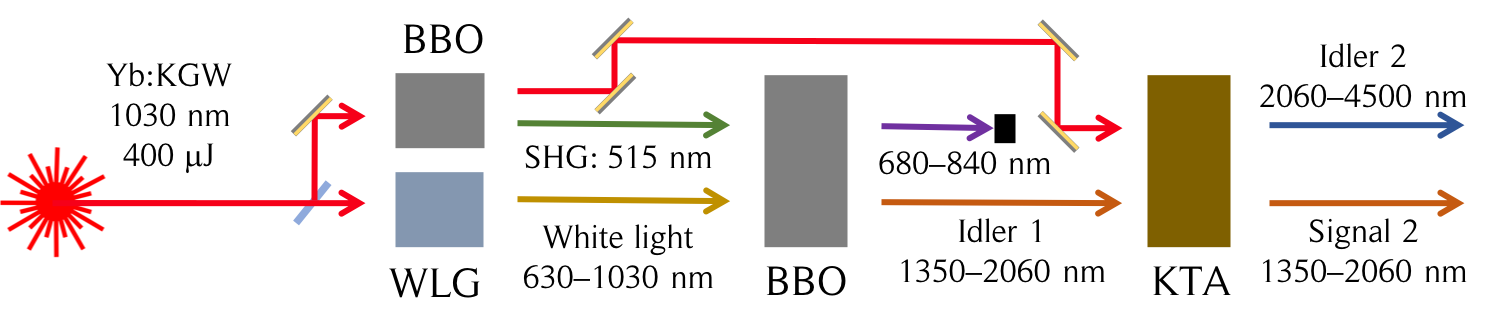
\includegraphics[width=1.0\figwidth]{chapters/Chapter3_Methods2/Graphs/PulsesScheme.png} %The local modes are calculated on the XXX level, and reproduced with permission from ref. XXX. 
	\caption{Schematic of the frequency conversion process to generate ultrafast IR pulses. BBO: barium borate crystal. WLG: white light generation substrate, sapphire. SHG: second harmonic generation. KTA: potassium titanyle arsenate crystal.}
	\label{UltraFastPulses}
\end{figure}






\subsection{Pump-probe optical setup}

As discussed previously in Section \ref{TRVSExp} and expressed in Eq.\ \ref{transientspectra1}, the aim of pump-probe spectroscopy is to measure the time-dependent changes in absorption as a given sample is perturbed by an intense pump pulse. The experimental setup consists of the following elements: pump pulses, probe pulses, a time-modulation translational stage and an IR sensitive detector. A schematic of the setup is shown in Figure~\ref{PumpProbeSetup}.

After setting the laser at the desired frequency, the beam (p-polarized) is directed to a \ce{ZnSe} beam splitter at an incident angle of 45$^o$, which transmits most of the light ($\sim$90\%) to generate the pump beam. The reflected light is directed to a second \ce{ZnSe} beam splitter to form the probe and the reference beam. The pump beam is sent to a computer-controllable translational stage to modulate the pump-to-probe time delay. Using a zero-order $\lambda /$2 plate, the polarization of the pump beam is set to 45$^\circ$ with respect of that polarization of the probe and reference beams. To determine pumped and unpumped transient signals, a chopper blade at a frequency of 500 Hz is placed in the pump optical path. Two wire-grid linear polarizers are used, one for the reference and one for the probe, to filter out undesired perpendicular or elliptical components. 


At this point, pump and probe are focused into the sample at the same spot, while the reference passes through the sample but does not overlap with the other beams. Directly after the sample, a rotating lineal polarizer is used to selectively filter out either the parallel or perpendicular components of the probe and the reference. This enables measurements to be taken in a polarization-resolved manner. After this selective step, the pump beam is blocked, while probe and reference are directed into a grating-based spectrometer that disperses the light onto a 3$\times$32-pixel array MCT (mercury-cadmium-telluride) detector.


\begin{figure}[t!]
	\centering
	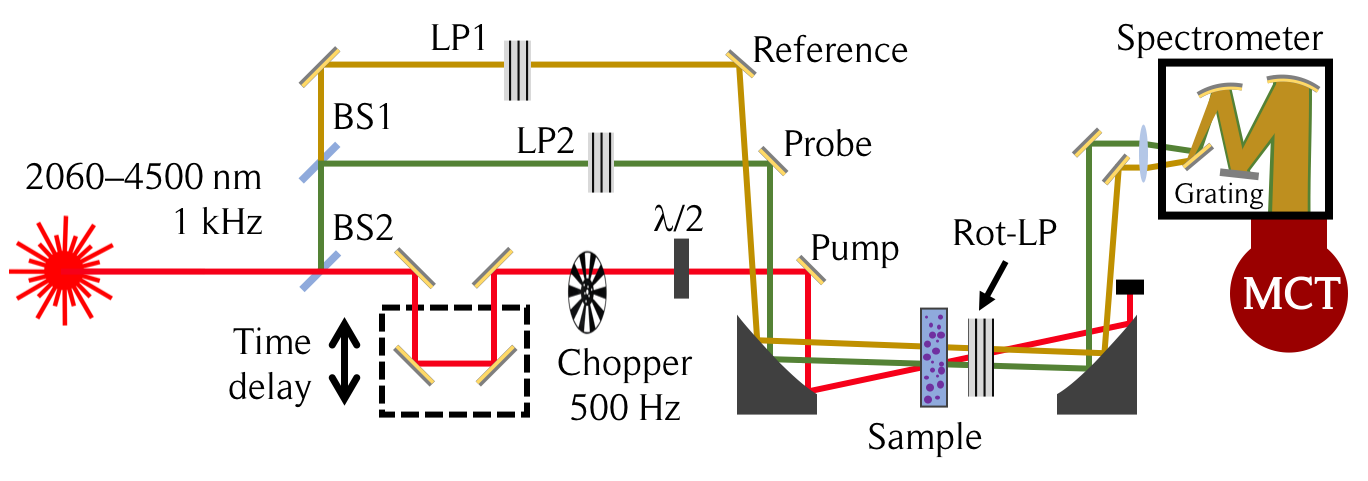
\includegraphics[width=1.0\figwidth]{chapters/Chapter3_Methods2/Graphs/PumpProbeSetup.png} %The local modes are calculated on the XXX level, and reproduced with permission from ref. XXX. 
	\caption{Schematic of the pump-probe optical setup. BS: \ce{ZnSe} beam splitter, LP: wire-grid linear polarizer, $\lambda/2$: zero-order half-wave plate, Rot-LP: rotational wire-grid linear polarizer, MCT: mercury-cadmium-telluride detector.}
	\label{PumpProbeSetup}
\end{figure}



The intensity of the probe is normalized with the intensity of the reference, and the transient absorption change is given by
\begin{eqnarray}
\Delta \alpha (\omega, t ) = - \ln   \underbrace{   \left[  \frac{I_\text{probe} (\omega,t)}{I_\text{ref} (\omega, t)}  \right] }_{\text{pumped}}  +  \ln  \underbrace{ \left[  \frac{I_\text{probe,0} (\omega,t)}{I_\text{ref,0} (\omega, t)}   \right] }_{\text{unpumped}} ,
\end{eqnarray}
which leads to 
\begin{eqnarray}
\nonumber \\
\Delta \alpha (\omega, t ) = - \ln \left[   \frac{I_\text{probe} (\omega,t)}{I_\text{ref} (\omega, t)}        \frac{I_\text{ref,0} (\omega, t)}{I_\text{probe,0} (\omega,t)}         \right] .
\end{eqnarray}

The preceding equation enables us to correct for shot-to-shot intensity fluctuations of the probe. This relation holds valid for both parallel and perpendicular transient absorption.


\section{Data analysis and modeling}\label{TRVSModel}


In this section we describe the the procedures used to extract information from our pump-probe experimental data. The transient signal is characterized by an excited state that decays ultimately into a hot ground state. However, the relaxation mechanism can be quite complicated, since the relaxation process may involve intermediate states. In aqueous solutions, additional excitation may appear due to the inhomogeneities caused by the solutes. One can often distinguish hydration water molecules from those which are far from any ion and behave in a bulk-like manner. In general, ions generate strong local electric field that change the spectra and relaxation rates of vibrations in their immediate vicinity. Therefore, the pump pulse might excite different vibrations at the same time, leading to a complicated spectral response.


We build up the analysis starting with the isotropic signal $\Delta \alpha_{\text{iso}}$, which is insensitive to molecular reorientation. We assume that the relaxation process consists of a linear combination of discrete relaxation steps, where each level is associated to a different spectral component with different population dynamics. As such, we can write
\begin{eqnarray}
\Delta \alpha_{\text{iso}} (\omega, t) = \sum_{i=1}^n \Delta\sigma_i({\omega}) N_i (t),
\label{linearcombiso}
\end{eqnarray}
with $\Delta\sigma_i$ the spectral signature of each constituent component and $N_i$ its corresponding population dynamics. The factor $n$ represents the number of energy levels that the relaxation mechanism possesses.

For the simplest relaxation mechanism, a two-level system, the population dynamics can be represented by the following set of differential equations
\begin{eqnarray}
\frac{d}{d t} \left( \begin{array}{c} N_1 (t) \\ N' (t) \end{array} \right) = \left( \begin{array}{cc} -k_1 & 0 \\ +k_1 & 0 \end{array} \right)  \left( \begin{array}{c} N_1 (t) \\ N' (t) \end{array} \right) \qquad \text{with} \qquad N_i(0) = \left( \begin{array}{c} N_1(0) \\ 0 \end{array} \right),
\label{simplestmodel}
\end{eqnarray}
where $N_1$ and $N'$ refer to the population dynamics of the excited and a final state that is not necessarily the ground state, and the relaxation rate $k_1$ is the reciprocal of the vibrational lifetime $T_1$. Solving these equation leads to the following description
\begin{eqnarray}
\Delta \alpha_{\text{iso}} (\omega, t) = \Delta\sigma_1 (\omega) N_1(0) e^{-k_1 t}  + \Delta\sigma' (\omega) N_1 (0)\left( 1 - e^{-k_1 t} \right),
\end{eqnarray}
where $\Delta \sigma_1 (\omega) = -2 \sigma_{10} (\omega) + \sigma_{21} (\omega)$ is the transient spectral response of the excited state, and $\Delta\sigma' = \sigma'_{10}(\omega) - \sigma_{10} (\omega)$ associated with the final state, as described in Eqs.\ \ref{transientspectra1} and \ref{transientabs2}. This relaxation mechanism is represented in the left side of Figure~\ref{simplestschem}.



\begin{figure}[t!]%* is used because without it the figure does not appear
	\centering	
	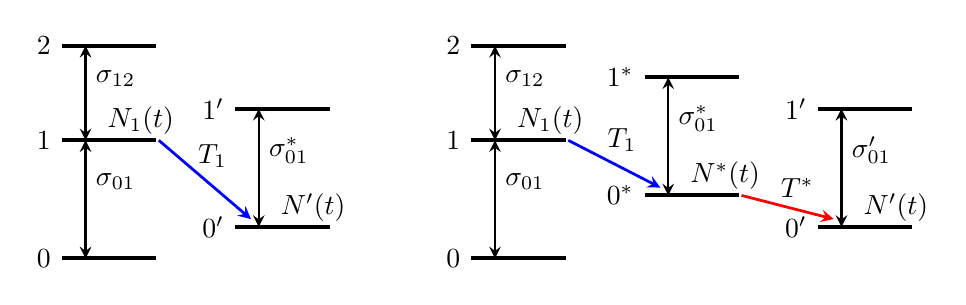
\begin{tikzpicture}[>=stealth,thick]	
	
	%\draw[white,line width=0.05mm](6,4) -- (7.5,4);
	
	\draw[->, line width=0.35mm, blue] (5.03,2.5) -- (6.2,1.9) ;
	\draw[->, line width=0.35mm, red] (7.23,1.8) -- (8.4,1.5);
	
	\draw[<->, line width=0.3mm, black] (4.1,1) -- (4.1,2.5) node[pos=0.65,right] {$\sigma_{01}$};
	\draw[<->, line width=0.3mm, black] (4.1,2.5) -- (4.1,3.7) node[pos=0.65,right] {$\sigma_{12}$};
	
	\draw[<->, line width=0.3mm, black] (6.3,1.8) -- (6.3,3.3) node[pos=0.65,right] {$\sigma_{01}^*$};
	
	\draw[<->, line width=0.3mm, black] (8.5,1.4) -- (8.5,2.9) node[pos=0.65,right] {$\sigma'_{01}$};
	
	\draw[black,line width=0.5mm](3.8,3.7) -- (5,3.7) node[pos=0.0,left] {$\ket{2}$};
	\draw[black,line width=0.5mm](3.8,2.5) -- (5,2.5) node[pos=0.0,left] {$\ket{1}$};
	\draw[black,line width=0.5mm](3.8,1.0) -- (5,1.0) node[pos=0.0,left] {$\ket{0}$};
	
	\draw[black,line width=0.5mm](6,3.3) -- (7.2,3.3) node[pos=0.0,left] {$\ket{1^*}$};
	\draw[black,line width=0.5mm](6,1.8) -- (7.2,1.8) node[pos=0.0,left] {$\ket{0^*}$};
	
	\draw[black,line width=0.5mm](8.2,2.9) -- (9.4,2.9) node[pos=0.0,left] {$\ket{1'}$};
	\draw[black,line width=0.5mm](8.2,1.4) -- (9.4,1.4) node[pos=0.0,left] {$\ket{0'}$};
	
	\node[right,align=left] at (5.4,2.5) {$T_1$};
	\node[right,align=left] at (7.6,1.9) {$T^*$};
	
	
	\node[right,align=left] at (4.25,2.75) {$N_1 (t)$};
	\node[right,align=left] at (6.45,2.05) {$N^* (t)$};
	\node[right,align=left] at (8.65,1.65) {$N' (t)$};
	
	
	
	
	\draw[->, line width=0.35mm, blue] (5.03-5.2,2.5) -- (6.2-5.2,1.5) ;	
	
	
	\draw[black,line width=0.5mm](3.8-5.2,3.7) -- (5-5.2,3.7) node[pos=0.0,left] {$\ket{2}$};
	\draw[black,line width=0.5mm](3.8-5.2,2.5) -- (5-5.2,2.5) node[pos=0.0,left] {$\ket{1}$};
	\draw[black,line width=0.5mm](3.8-5.2,1.0) -- (5-5.2,1.0) node[pos=0.0,left] {$\ket{0}$};
	
	\draw[black,line width=0.5mm](6-5.2,2.9) -- (7.2-5.2,2.9) node[pos=0.0,left] {$\ket{1'}$};
	\draw[black,line width=0.5mm](6-5.2,1.4) -- (7.2-5.2,1.4) node[pos=0.0,left] {$\ket{0'}$};
	
	
	\draw[<->, line width=0.3mm, black] (4.1-5.2,1) -- (4.1-5.2,2.5) node[pos=0.65,right] {$\sigma_{01}$};
	
	\draw[<->, line width=0.3mm, black] (4.1-5.2,2.5) -- (4.1-5.2,3.7) node[pos=0.65,right] {$\sigma_{12}$};
		
	\draw[<->, line width=0.3mm, black] (6.3-5.2,1.4) -- (6.3-5.2,2.9) node[pos=0.65,right] {$\sigma_{01}^*$};
	
	
	\node[right,align=left] at (4.25-5.2,2.75) {$N_1 (t)$};
	\node[right,align=left] at (6.45-5.2,1.65) {$N' (t)$};
%	\node[right,align=left] at (8.65,1.65) {$N' (t)$};
	
	\node[right,align=left] at (5.4-5.2,2.3) {$T_1$};
	
	%\draw[white,line width=0.05mm](1,-0.1) -- (7,-0.1);
	
	\end{tikzpicture}		
	\caption{\textbf{Left:} One-step relaxation mechanism in which the excited oscillators relax directly to a final state (not necessarily the original ground state). \textbf{Right:} Two-step relaxation mechanism in which the excited oscillators decay first to an intermediate state, before attaining the final equilibrium state. The difference between the final state and the original ground state accounts for irreversible changes or heating in the sample due to the intense pump pulse.}
	\label{simplestschem}			
\end{figure}



Unfortunately, the vibrational relaxation process in aqueous systems is never this simple. It has been demonstrated that the vibrational relaxation dynamics of \ce{OD}/\ce{OH} stretch vibrations in isotopically diluted \ce{H2O}/\ce{D2O} is well described by a two-step consecutive model as shown in the right side of Figure~\ref{simplestschem},\!\cite{Rezus2005,Rezus2006} in which the population dynamics are represented with the following differential equations
\begin{eqnarray}
\frac{d}{d t} \left( \begin{array}{c} N_1 (t)\\ N^* (t) \\ N' (t) \end{array} \right) = \left( \begin{array}{ccc} -k_1 & 0 & 0 \\ +k_1 & -k^* & 0 \\ 0 & +k^* & 0 \end{array} \right)  \left( \begin{array}{c} N_1 (t) \\ N^* (t) \\ N' (t) \end{array} \right),
\label{cascademodel}
\end{eqnarray}
where the initial conditions are $N_i (0) = \left(  N_1 (0), 0 , 0   \right)$. In this model, the system relaxes via an intermediate state $\ket{0^*}$ to the hot ground state $\ket{0'}$. 
%In this case, the intermediate state is associated only with a retarded response of the thermal state, with respect to the fast vibrational relaxation. In other words, the coordinates of the hydrogen-bond network take a finite time $T_* = 1/k_*$ to equilibrate with the resulting vibrations from the relaxation process. As such, 
It has been found previously that the intermediate state has the same spectrum as the ground ground state ($\sigma_{01}^* = \sigma_{01}$), meaning that the intermediate state has no associated transient spectrum. In this case, the isotropic transient signal can be model as
\begin{eqnarray}
\Delta \alpha_{\text{iso}} (\omega, t) &=& \Delta\sigma_1 (\omega) N_1(0) e^{-k_1 t} \nonumber \\ &+& \Delta\sigma' (\omega) N_1(0)\left( 1 + \frac{k_1}{k^* - k_1} e^{-k^* t} - \frac{k^*}{k^* - k_1} e^{-k_1 t} \right),
\label{Solutioncascademodel}
\end{eqnarray}
with $\Delta\sigma_1 (\omega) = -2 \sigma_{10} (\omega) + \sigma_{21} (\omega)$ the transient signal of the excited state, and $\Delta\sigma' = \sigma'_{10}(\omega) - \sigma_{10} (\omega)$ the transient signal associated with the hot ground state.


For more complex models, providing a solution to the set of differential equations becomes complicated and tedious for numerical analyses. A easier solution consists of diagonalizing the rate matrix $K$ of the Eqs.\ \ref{simplestmodel} and \ref{cascademodel} written in matrix form as
\begin{eqnarray}
\frac{d}{d t} \vec{N} = K \vec{N}.
\label{differentialK}
\end{eqnarray}

We aim to find a unitary matrix $U$ such that $K U = U \lambda$,
%\begin{eqnarray}
%K U = U \lambda,
%\label{eigenEq2}
%\end{eqnarray}
where $\lambda$ is a diagonal matrix that contains the eigenvalues and $U$ contains the vectors that form the eigenbasis. %In line with this description, the vector $\vec{N}$ corresponds to another as
%\begin{eqnarray}
%\vec{N} (t) = U \vec{M} (t), \qquad \text{where} \qquad \vec{N} (0) = U \vec{M} (0)
%\label{transVector}
%\end{eqnarray}
%holds valid. By using 
%Combining Eqs.\ \ref{differentialK} and \ref{eigenEq2}, we obtain 
As such, the population dynamics are given by
\begin{eqnarray}
\vec{N} (t) = U \exp(\lambda t) U^{-1} \vec{N} (0),
\label{PopuEigen}
\end{eqnarray}
which offers a general solution as a linear combination of exponential decays in terms of the eigenvalues of the rate matrix $K$.



To extract meaningful information from the experimental data $\Delta\alpha_\text{iso}^\text{exp} (\omega,t)$ with standard deviation $\xi (\omega, t)$, we perform least-squares fits to minimize the following weighted $\chi^2$ function
\begin{eqnarray}
\chi^2 = \int \int \left( \frac{\Delta \alpha_\text{iso}^\text{exp} (\omega,t) - \sum_i \Delta\sigma_i(\omega)N_i(t)}{\xi (\omega, t)}\right)^2 dt d\omega,
\label{ChiSquare}
\end{eqnarray}
in which the spectral components $\Delta\sigma_i$ and the decay rate constants \textbf{k} are treated as fit parameters.
%in general, we need a large amount of fitting parameters. However, we aim to find information that allow us to reduce the number of fitting parameters. 


If one knows the relaxation mechanism $K(\text{\textbf{k}})$, the time traces $\vec{N}$ are determined by the \textbf{k} parameters, and we can find the spectral components that minimize the $\chi^2$ function at all times. This method is usually called spectral decomposition. This approach starts out with an estimate for the decay rates \textbf{k}, from which a subsequent minimization process finds the spectral signatures that best fit the experimental data following the expression
\begin{eqnarray}
\frac{d}{d \tilde{\sigma}_i (\omega)} \int \left( \frac{\Delta \alpha_\text{iso}^\text{exp} (\omega,t) - \sum_i \Delta\tilde{\sigma}_i(\omega)N_i(\textbf{k},t)}{\xi (\omega, t)}\right)^2 dt = 0
\label{SpectralDecomp}
\end{eqnarray}
to find the optimal decay rates \textbf{k}. A minimization routine following this approach is shown in Listing \ref{Listing2} using the kinetic model from Eq.\ \ref{cascademodel}.


Analogously, if one knows the spectral components $\Delta\sigma_i$, one can run a minimization process to extract the time traces that best fit the experimental data. This approach is called temporal decomposition, and from
\begin{eqnarray}
\frac{d}{d \tilde{N}_i (t)} \int \left( \frac{\Delta \alpha_\text{iso}^\text{exp} (\omega,t) - \sum_i \Delta\sigma_i(\omega) \tilde{N}_i(t)}{\xi (\omega, t)}\right)^2 d\omega = 0,
\label{TemporalDecomp}
\end{eqnarray}
we obtain the population dynamics. This approach is more convenient for the study of samples in which unconventional processes, such as F\"orster resonance energy transfer,\!\cite{Forster1948} play an important role in the relaxation dynamics. A complete analysis of experimental data that show a F\"orster-like relaxation process is available at \href{https://github.com/RobertoCota/Forster-energy-transfer}{https://github.com/RobertoCota/Forster-energy-transfer}

To extract information on the molecular reorientation dynamics, we use Eqs.\ \ref{isotropicsignal}, \ref{anisotropysignal} and \ref{linearcombiso} to define the following equations
\begin{eqnarray}
\Delta \alpha_\parallel (\omega, t) &=& \sum_{i=i}^n [1 + 2 R_i(t)] N_i (t) \Delta\sigma_i(\omega) = \sum_{i=1}^n N_{i,\parallel} (t) \Delta\sigma_i (\omega) \\
\Delta \alpha_\perp (\omega, t) &=& \sum_{i=i}^n [1 -  R_i(t)] N_i (t) \Delta\sigma_i(\omega) = \sum_{i=1}^n N_{i,\perp} (t) \Delta\sigma_i (\omega),
\end{eqnarray}
in which we associate an anisotropy $R_i (t)$ with each spectral component. To this purpose, we can perform a temporal decomposition minimization on both parallel and perpendicular signals. Having retrieved $N_{i,\parallel} (t)$ and $N_{i,\perp} (t)$, we can calculate the anisotropy of each constituent component as
\begin{eqnarray}
R_i(t) = \frac{N_{i,\parallel} (t) - N_{i,\perp} (t)}{ N_{i,\parallel} (t) + 2 N_{i,\perp} (t)}.
\end{eqnarray}

A global minimization is possible by performing a least-square routine to minimize the following $\chi^2$ function
\begin{eqnarray}
\begin{split}
\chi^2 = \int \int   dt d\omega \left[    \left( \frac{\Delta \alpha_\parallel^\text{exp} (\omega,t) - \sum_i [1 + 2 R_i(t)]N_i(t) \Delta\sigma_i(\omega)}{\xi_\parallel (\omega, t)}\right)^2 \right. \\ \left. +     \left( \frac{\Delta \alpha_\perp^\text{exp} (\omega,t) - \sum_i [1 - R_i(t)]N_i(t) \Delta\sigma_i(\omega)}{\xi_\perp (\omega, t)}\right)^2  \right]  
\label{ChiSquareGlobal}
\end{split}
\end{eqnarray}
where parallel and perpendicular signals are minimized simultaneously. As shown in Chapter \ref{ChapterHydroxide}, this equation can be used to perform spectral decomposition if one defines the relaxation pathway and assign functional forms to each $R_i$ component. An example of this type of analysis is available at \href{https://github.com/RobertoCota/Time-resolved-vibrational-spectroscopy}{https://github.com/RobertoCota/Time-resolved-vibrational-spectroscopy}.


%\newpage
\bigskip
\bigskip

\lstinputlisting[language=Python,caption={Python script for the analysis of isotropic transient absorption in which a two-step consecutive model, represented by Eqs.~\ref{cascademodel} and \ref{Solutioncascademodel}, is used.},label={Listing2}]{chapters/Chapter3_Methods2/Graphs/SpectralDecomposition.py}


